% !TEX root = Master.tex

The next step, after fitting proper models to the marginal distributions of the log-sales aggregated on key category cluster level, is to enter the pairwise modelling of the clusters. Specifically, we are interested in capturing the dependence structure over time which is delineated in the next three Subsections (\ref{sssec:kcc_26}, \ref{sssec:kcc_28} and \ref{sssec:kcc_68}).
\\

%Recalling the previous Section \ref{ssec:kcc_marginals}, the residuals from the fitting method are depicted in \autoref{fig:res_gamlss_over_time} for each time-point.

%\begin{figure}[H]
%\centering
%  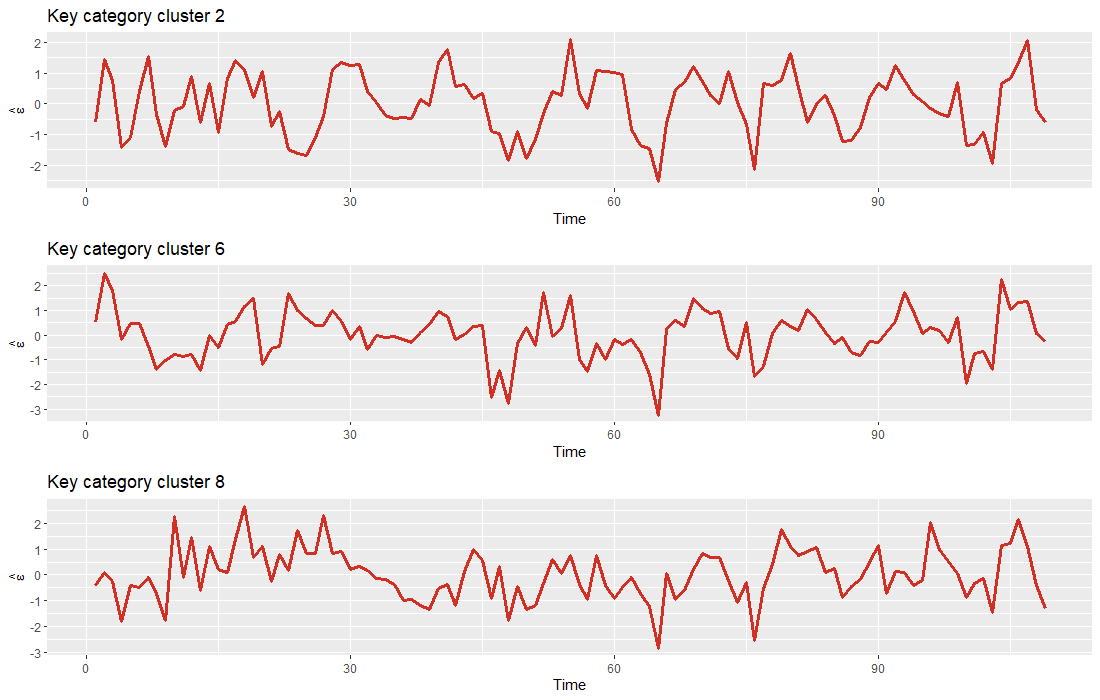
\includegraphics[width=0.95\linewidth]{figures/res_gamlss_over_time.png}
%  \caption{Estimated residuals of GAMLSS fits for the three key category clusters}
%  \label{fig:res_gamlss_over_time}
%\end{figure}